%% 2019 NeuroFedora contributors

%% packages %%
% support for coloured text
\usepackage{xcolor}
\definecolor{FedoraBlue}{cmyk}{1.0,0.46,0.0,0.0}
\definecolor{FedoraDarkBlue}{cmyk}{1.0,0.57,0.0,0.38}
\definecolor{FriendsMagenta}{cmyk}{0.0,0.8,0.4,0.0}
\definecolor{FeaturesOrange}{cmyk}{0.0,0.5,1.0,0.0}
\definecolor{FirstGreen}{cmyk}{0.5,0.0,1.0,0.0}
\definecolor{FreedomPurple}{cmyk}{0.57,0.46,0.0,0.0}

% IPA
\usepackage{tipa}
\usepackage[scale=2]{ccicons}
\usepackage{amssymb}
\usepackage{tikz}
\usetikzlibrary{arrows.meta, arrows, positioning}
\usepackage{jneurosci}
\usepackage{subfig}
\usepackage[T1]{fontenc}
\usepackage[utf8]{inputenc}
\usepackage[style=verbose,backend=biber,autocite=footnote]{biblatex}
\addbibresource{masterbib.bib}
% Use opensans
\usepackage[default,osfigures,scale=0.95]{opensans}
% for strike through
\usepackage[normalem]{ulem}
% links, urls, refs
\usepackage{hyperref}
\hypersetup{colorlinks,linkcolor=FreedomPurple,urlcolor=FreedomPurple}
% graphics
\usepackage{graphicx}
% algorithm
\usepackage{algorithmic}
\usepackage{textcomp}
\usepackage{wrapfig}
\usepackage{textgreek}
\usepackage{euler}
\usepackage{ccicons}
\usepackage{pdfpages}
% \usepackage{minted}

% beamer theme
\usetheme[numbering=fraction]{metropolis}
\usefonttheme[onlymath]{serif}
\setbeamerfont{footnote}{size=\tiny}
\setbeamerfont{caption}{size=\tiny}
\setbeamercolor{alerted text}{fg=FeaturesOrange}
\setbeamercolor{progress bar}{fg=FriendsMagenta}
\setbeamercolor{title separator}{fg=FriendsMagenta}
\setbeamercolor{frametitle}{bg=FedoraDarkBlue}

\renewcommand{\figurename}{}

% Not needed in metropolis, but in general footnote citation fixes: https://tex.stackexchange.com/questions/44217/how-can-i-stop-footcite-from-hijacking-my-beamer-columns
% how to use multiple references to the same footnote: https://tex.stackexchange.com/questions/27763/beamer-multiple-references-to-the-same-footnote

%% title %%
\title[Journal club]{Standards and Tools in Neuroscience}
\subtitle{A summary of the Open Source Brain workshop, September 2019}
\author{Ankur Sinha\\Ph.D. candidate: UH Biocomputation Group, UK,\\Volunteer: Fedora Project.}
\date[]{}
%% document begins %%
\begin{document}

% title frame %%
\begin{frame}
  \titlepage{}
\end{frame}

%% 3 slides for 5 minutes, so 30 slides for 45 minutes.
\section{The problem statement}
\begin{frame}[c]{Neuroscience is complex, and massive}
  \begin{figure}[h]
    \centering
    \only<1>{\tikzset{
    %Define standard arrow tip
    >=stealth',
    %Define style for boxes
    punkt/.style={
           circle,
           draw=black, very thick,
           text=FedoraDarkBlue,
           text width=6em,
           minimum height=2em,
           text centered},
    % Define arrow style
    pil/.style={
           <-,
           very thick,
           draw=FreedomPurple,
           shorten <=2pt,
           shorten >=2pt,}
}
\begin{tikzpicture}[node distance=1cm, auto,]
 %nodes
 \node[punkt, draw=FedoraBlue, text=FedoraBlue] (experiments) {Experimental work};
 \node[punkt, draw=FriendsMagenta, text=FriendsMagenta, above right=of experiments]
 (analysis) {Data analysis}
 edge[pil, bend right=45] (experiments.north);
 \node[punkt, draw=FeaturesOrange, text=FeaturesOrange, below right=of analysis]
 (theory) {Theory}
 edge[pil, bend right=45] (analysis.east);
 \node[punkt, draw=FirstGreen, text=FirstGreen, below left=of theory]
 (modelling) {Modelling}
 edge[pil, bend right=45] (theory.south)
 edge[pil, ->, bend left=45] (experiments.south);
 % We make a dummy figure to make everything look nice.
 % \node[above=of market] (dummy) {};
 % \node[right=of dummy] (t) {Ultimate borrower}
   % edge[pil,bend left=45] (market.east) % edges are used to connect two nodes
   % edge[pil, bend left=45] (formidler.east); % .east since we want
                                             % % consistent style
 % \node[left=of dummy] (g) {Ultimate lender}
   % edge[pil, bend right=45] (market.west)
   % edge[pil, bend right=45] (formidler.west)
   % edge[pil,<->, bend left=45] node[auto] {Direct (a)} (t);
\end{tikzpicture}
}%
    \only<2>{\tikzset{
    %Define standard arrow tip
    >=stealth',
    %Define style for boxes
    punkt/.style={
           circle,
           draw=black, very thick,
           text=FedoraDarkBlue,
           text width=6em,
           minimum height=2em,
           text centered},
    % Define arrow style
    pil/.style={
           <-,
           very thick,
           draw=FreedomPurple,
           shorten <=2pt,
           shorten >=2pt,}
}
\begin{tikzpicture}[node distance=1cm, auto,]
 %nodes
 \node[punkt, draw=FedoraBlue, text=FedoraBlue] (experiments) {Experimental work};
 \node[punkt, draw=FriendsMagenta, text=FriendsMagenta, above right=of experiments]
 (analysis) {Data analysis}
 edge[pil, ->, bend left=45, opacity=0.4] (experiments.east)
 edge[pil, bend right=45] (experiments.north);
 \node[punkt, draw=FeaturesOrange, text=FeaturesOrange, below right=of analysis]
 (theory) {Theory}
 edge[pil, bend right=45] (analysis.east)
 edge[pil, ->, bend left=45, opacity=0.4] (analysis.south);
 \node[punkt, draw=FirstGreen, text=FirstGreen, below left=of theory]
 (modelling) {Modelling}
 edge[pil, bend right=45] (theory.south)
 edge[pil, ->, bend left=45] (experiments.south)
 edge[pil, ->, bend left=45, opacity=0.4] (theory.west)
 edge[pil, <-, bend right=45, opacity=0.4] (experiments.east)
 edge[pil, ->, bend left=45, opacity=0.4] (analysis.south)
 edge[pil, <-, bend right=45, opacity=0.4] (analysis.south);
 % We make a dummy figure to make everything look nice.
 % \node[above=of market] (dummy) {};
 % \node[right=of dummy] (t) {Ultimate borrower}
   % edge[pil,bend left=45] (market.east) % edges are used to connect two nodes
   % edge[pil, bend left=45] (formidler.east); % .east since we want
                                             % % consistent style
 % \node[left=of dummy] (g) {Ultimate lender}
   % edge[pil, bend right=45] (market.west)
   % edge[pil, bend right=45] (formidler.west)
   % edge[pil,<->, bend left=45] node[auto] {Direct (a)} (t);
\end{tikzpicture}
}
    \note[item]{A simplified diagram. Actually a lot more complex}
  \end{figure}
  \note[item]{It is so massive that you can speak to another neuroscientist and not understand a word of what they say---we specialise}
  \note[item]{We won't even discuss dissemination to a non scientific audience today---a completely different problem.}
\end{frame}
\begin{frame}[c]{Free/Open Neuroscience}
  Free/Open science:\\Scientific material should be easily, openly \alert{accessible to all}.
\end{frame}
{
  \setbeamercolor{background canvas}{bg=}
  \includepdf[pages={22,4,5}]{./2019-OSB-slides/OSB_introduction_Final_Angus.pdf}
}
\section{Standards: the common tongue}
{
  \setbeamercolor{background canvas}{bg=}
  \includepdf[pages={1,2,3,4,6,11,15,27,29,30}]{./2019-OSB-slides/2019_09_09_opensourcebrain_nwbn_overview.pdf}
  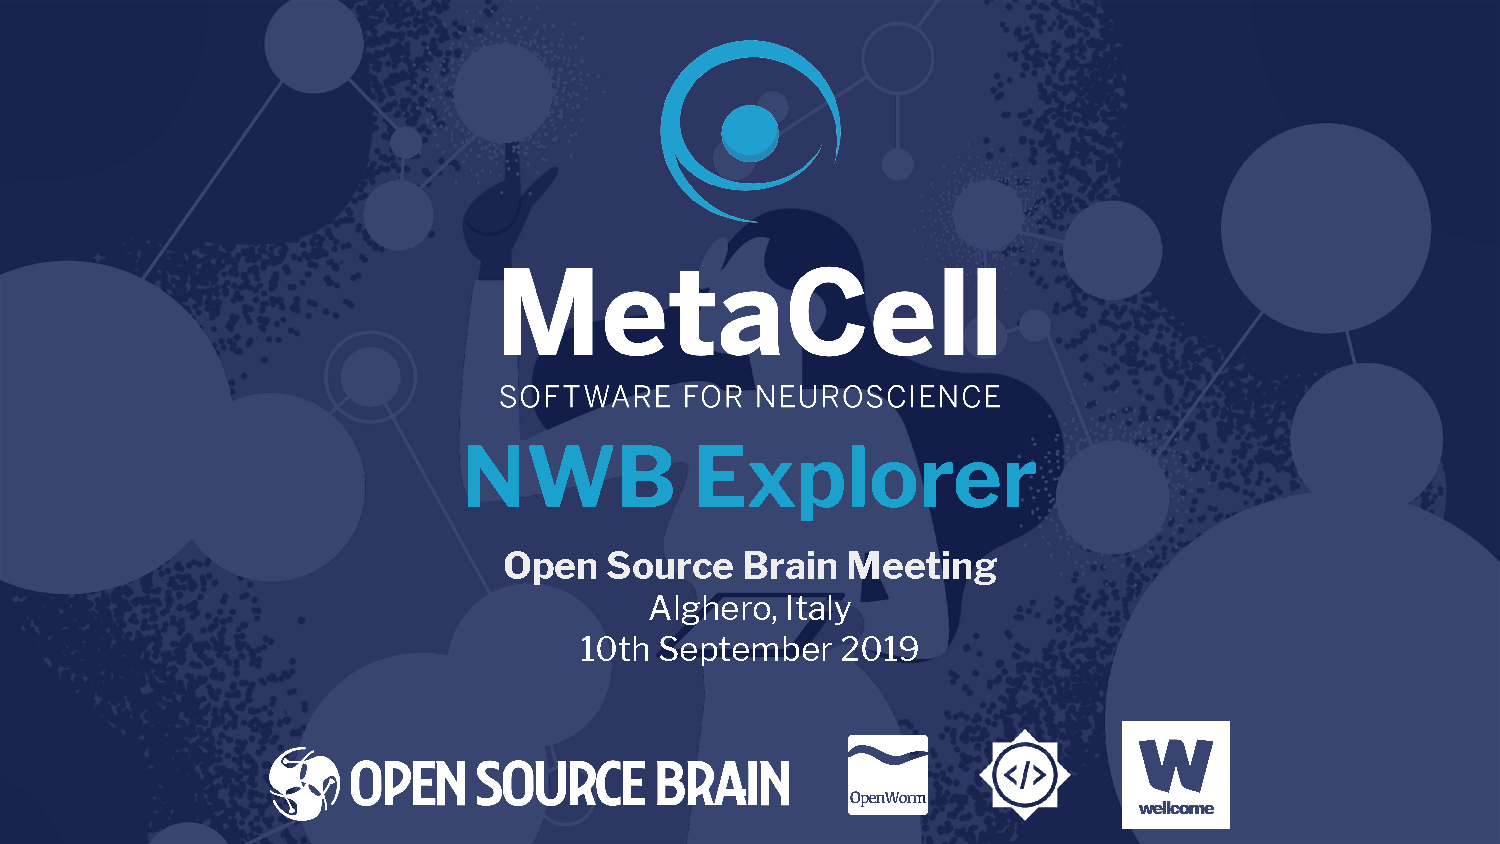
\includepdf[pages={1,5,7}]{./2019-OSB-slides/NWBExplorerOSBMeeting2019.pdf}
  \includepdf[pages={1,7,15,25,32,33}]{./2019-OSB-slides/MultiscaleNetworksNeuroML_Sardinia19.pdf}
  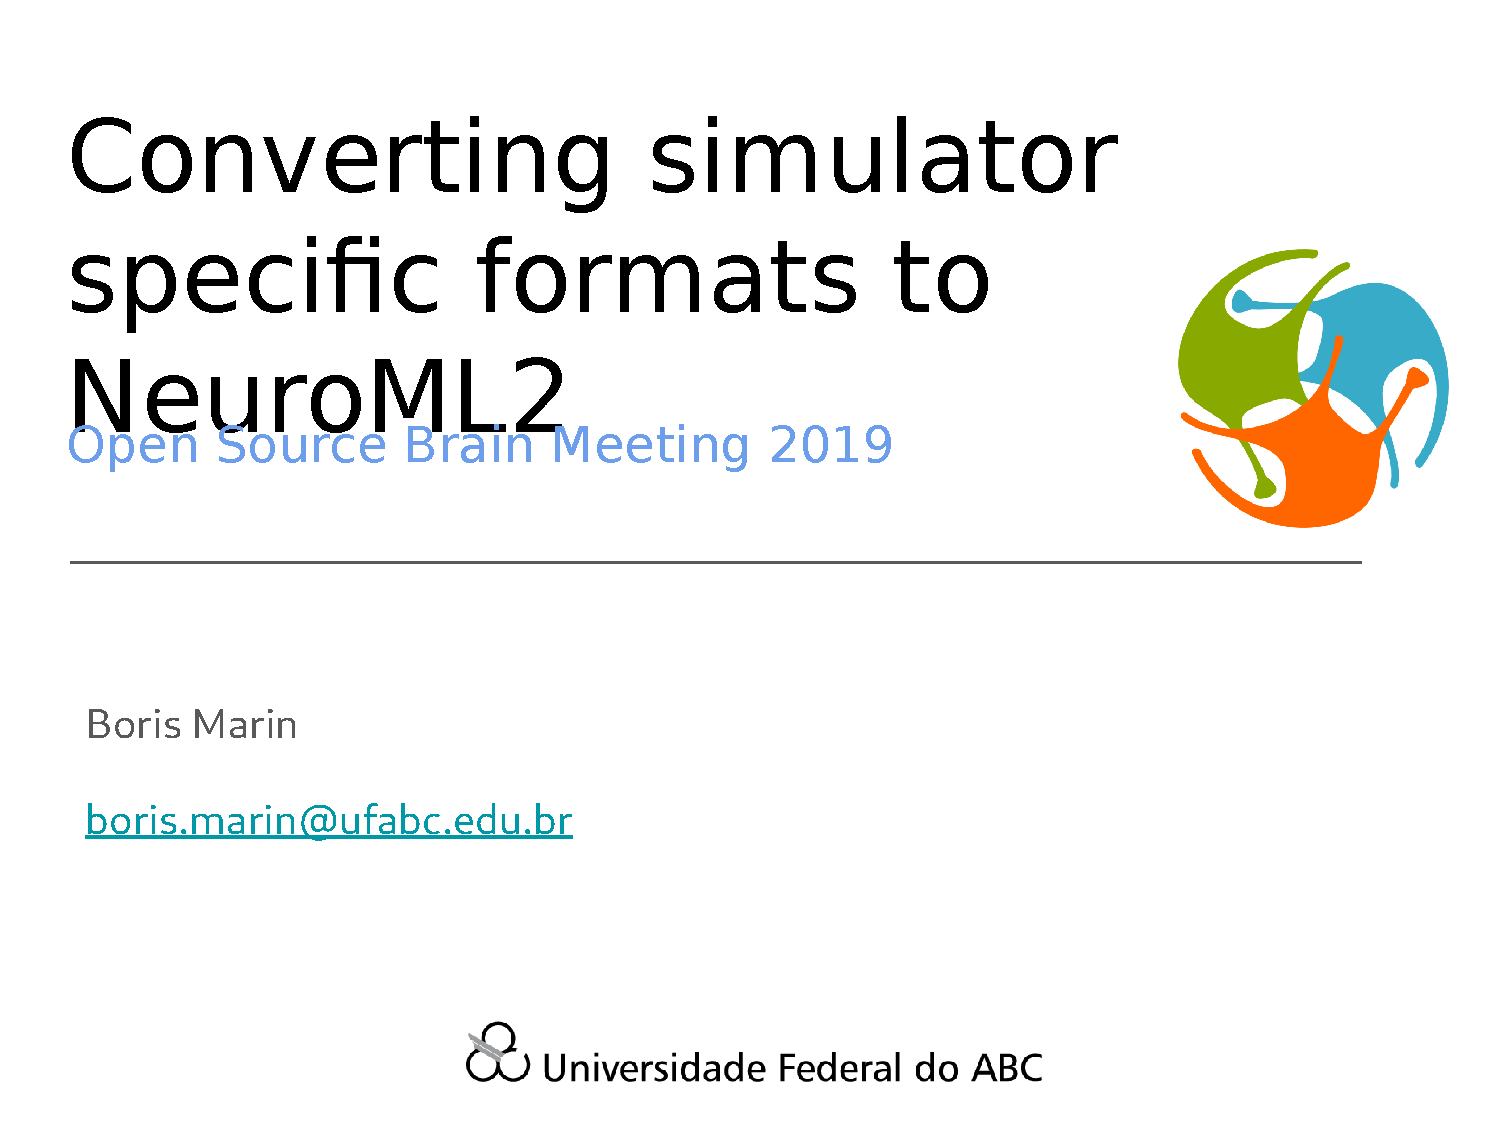
\includepdf[pages={1,2,7,8,9,10,11,13}]{./2019-OSB-slides/BorisMarin_Sardinia2019.pdf}
}
\begin{frame}[c]{Netpyne workflow}
  \begin{figure}[h]
    \centering
    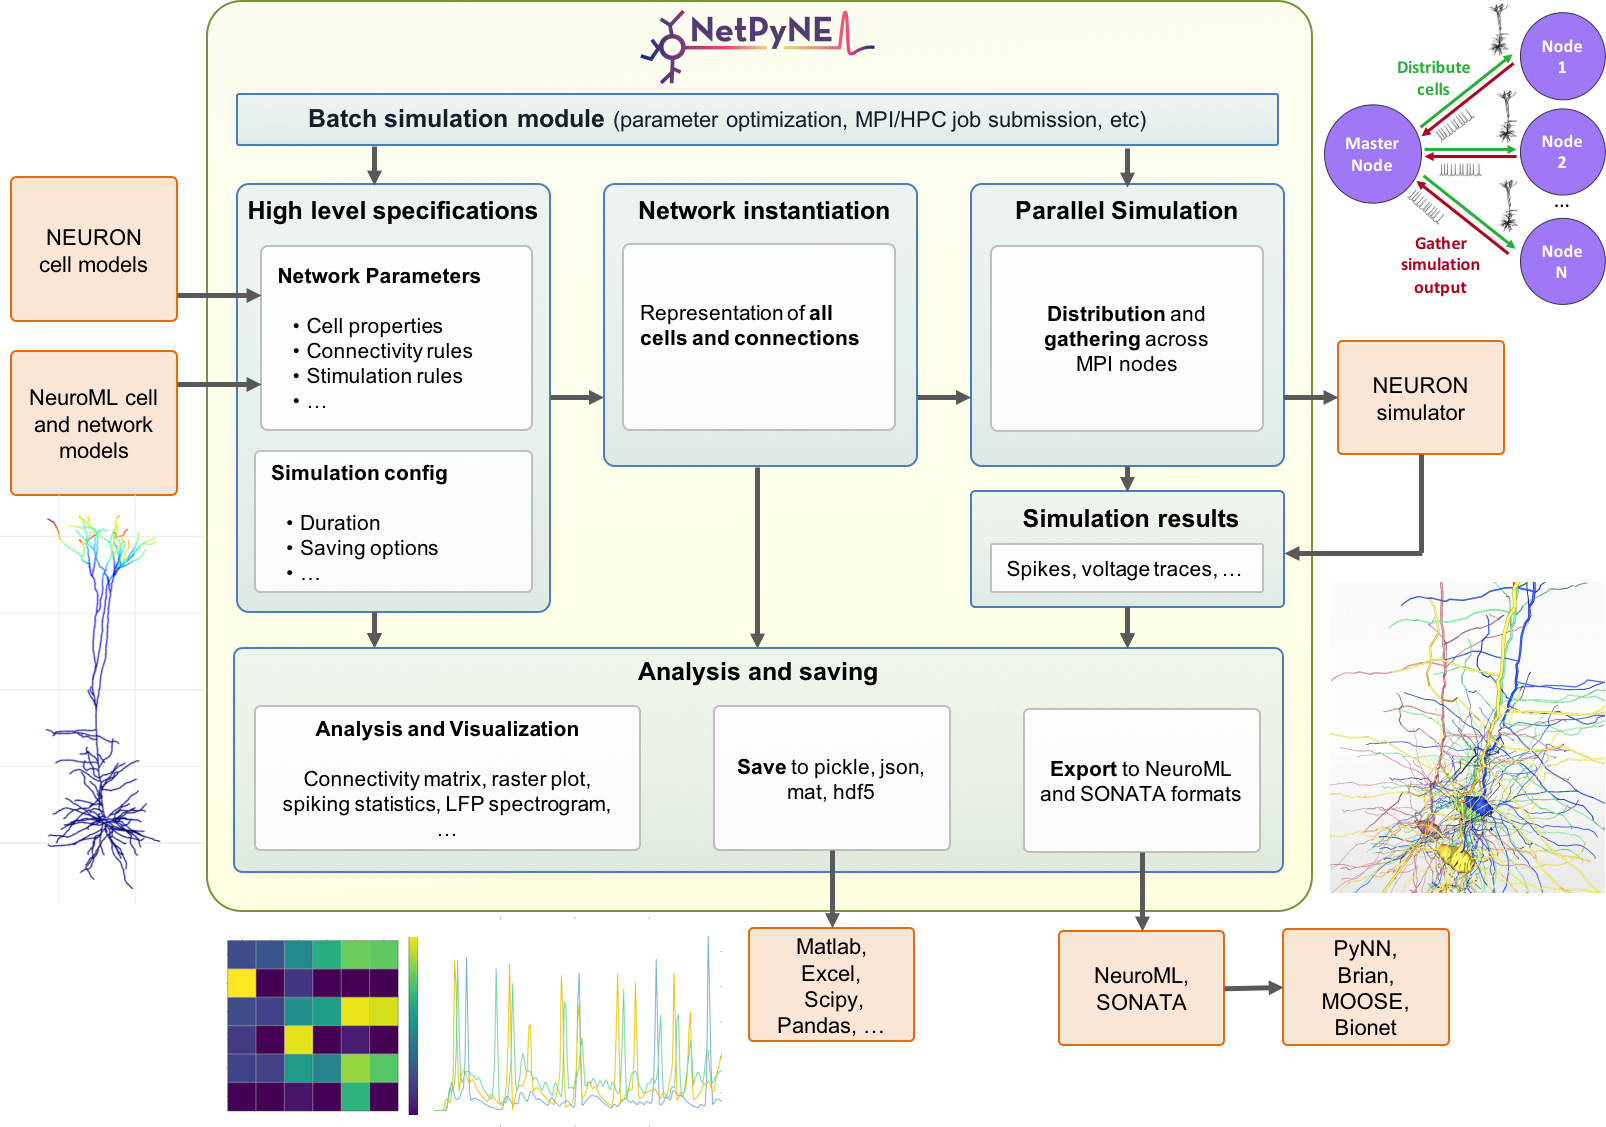
\includegraphics[width=\linewidth]{images/netpyne.png}
  \end{figure}
\end{frame}
\begin{frame}[c]{Netpyne GUI}
  \begin{figure}[h]
    \centering
    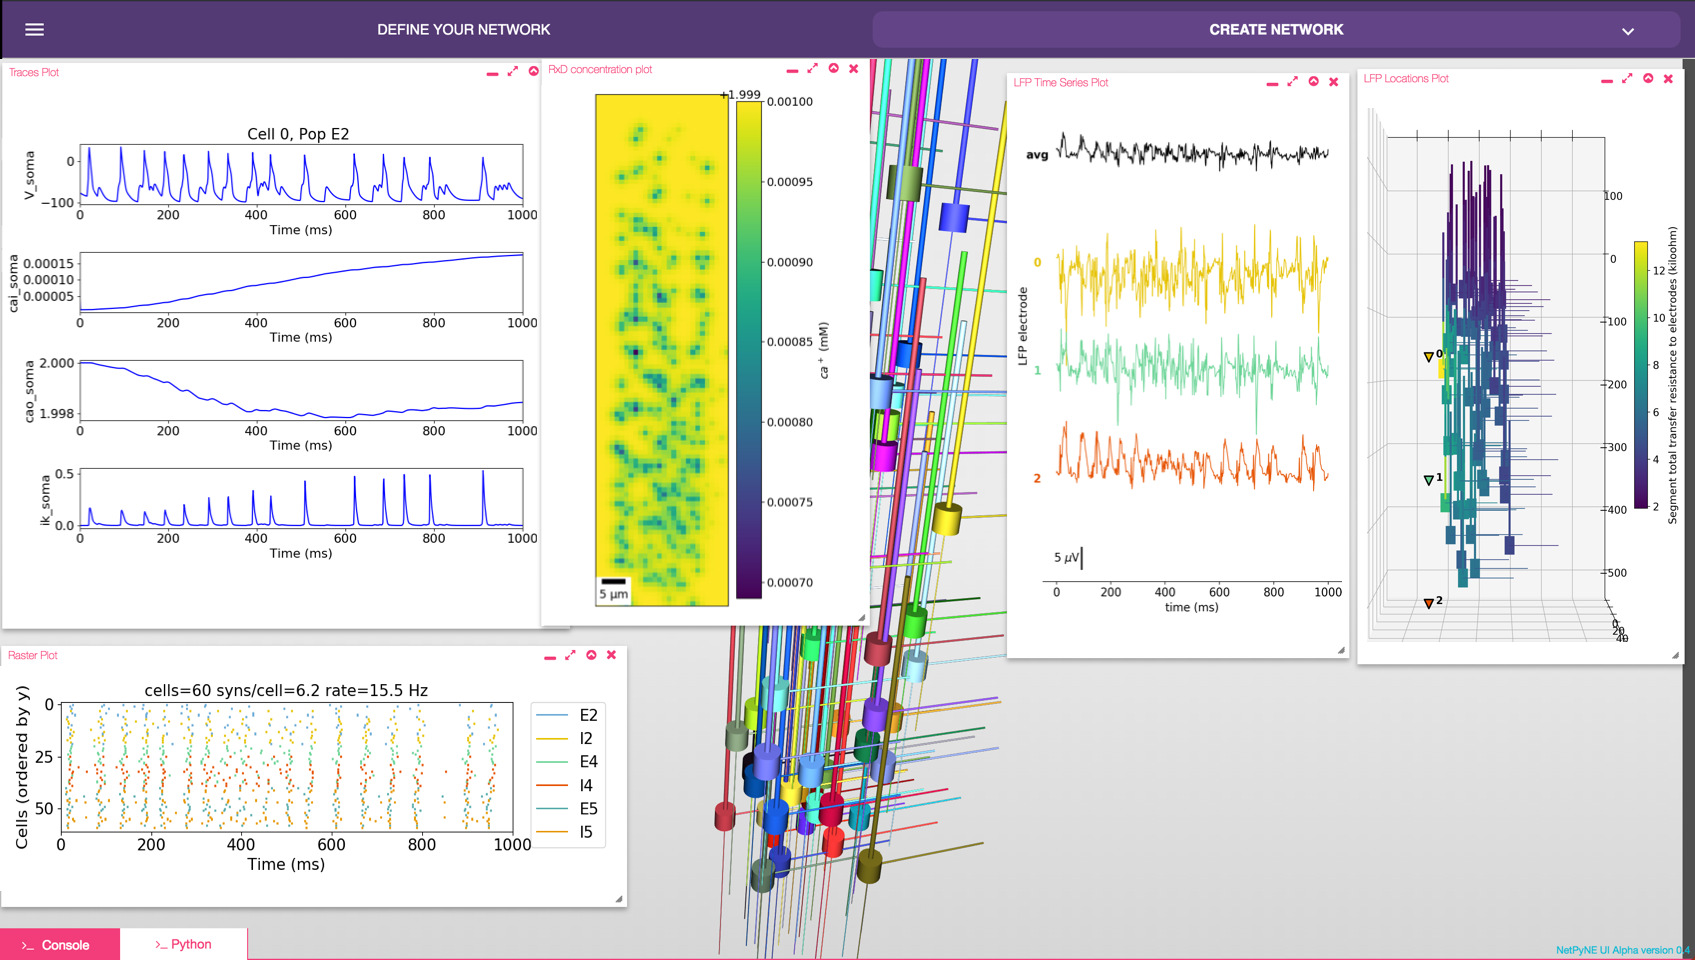
\includegraphics[width=\linewidth]{images/netpyne-gui.png}
  \end{figure}
\end{frame}
{
  \setbeamercolor{background canvas}{bg=}
  \includepdf[pages={1,2,3,4,25,26}]{./2019-OSB-slides/2019-09-OSB_YazanBilleh_v2.pdf}%chktex 8
  \includepdf[pages={1,3,7,8,9,23,29}]{./2019-OSB-slides/OSB_2019_yann.pdf}
}
\section{NeuroFedora: marketing pitch}
\begin{frame}[c]{Liaison between developers and users}
  \begin{figure}[h]
  \begin{center}
  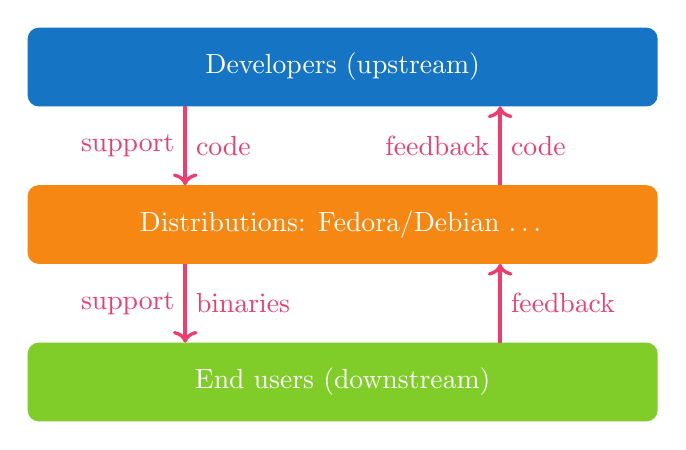
\begin{tikzpicture}[scale=1, transform shape]
    \fill[fill=FedoraBlue, text=white, rounded corners] (0, 0) rectangle ++(8, 1) node[pos=0.5] (A){Developers (upstream)};
    \fill[fill=FeaturesOrange, text=white, rounded corners] (0, -2) rectangle ++(8, 1) node[pos=0.5] (B){Distributions: Fedora/Debian \ldots};
    \draw [FriendsMagenta, very thick, ->] (2, 0) -- node [midway, right, text centered] {code} node [midway, left, text centered] {support} ++(0, -1) ;
    \draw [FriendsMagenta, very thick, ->] (6, -1) -- node [midway, right, text centered] {code} node [midway, left, text centered] {feedback} ++(0, 1) ;
    \fill[fill=FirstGreen, text=white, rounded corners] (0, -4) rectangle ++(8, 1) node[pos=0.5] (B){End users (downstream)};
    \draw [FriendsMagenta, very thick, ->] (2, -2) -- node [midway, right, text centered] {binaries} node [midway, left, text centered] {support} ++(0, -1) ;
    \draw [FriendsMagenta, very thick, ->] (6, -3) -- node [midway, right, text centered] {feedback} ++(0, 1) ;
  \end{tikzpicture}
  \end{center}
  \end{figure}
\end{frame}
\begin{frame}[c]{Search: \enquote{NeuroFedora}}
  \begin{columns}
   \begin{column}{0.3\textwidth}
      \begin{figure}[h]
        \centering
        
\includegraphics[width=\linewidth]{images/NeuroFedoraBadge.png}
      \end{figure}
    \end{column}
    \begin{column}{0.8\textwidth}
      \textcolor{FeaturesOrange}{\enquote{Live} ISO now ready to download (demo)}\\
      \textcolor{FedoraBlue}{Mailing list:\ neuro-sig@lists.fedoraproject.org}\\
      \textcolor{FirstGreen}{IRC:\ \#fedora-neuro on Freenode}\\
      \textcolor{FeaturesOrange}{Telegram:\ t.me/NeuroFedora}\\
      \textcolor{FriendsMagenta}{Documentation\ neuro.fedoraproject.org}\\
      \textcolor{FirstGreen}{Blog:\ neuroblog.fedoraproject.org}\\
      \textcolor{FeaturesOrange}{Pagure.io (FOSS Git forge):\ neuro-sig/NeuroFedora}
    \end{column}
  \end{columns}
\end{frame}
\begin{frame}[c]{License}
  \begin{center}
    \ccbysa{}\\
    \vspace{0.5cm}
    This presentation is made available under a \href{https://creativecommons.org/licenses/by-sa/4.0/}{Attribution-ShareAlike 4.0 International (CC BY-SA 4.0) license}.\\
  \end{center}
\end{frame}
\end{document}
